\chapter{Aplicaciones y calibración}
\section{Voltímetro}
Muestra la tensión de la batería durante el funcionamiento. evo\_v\_l presenta un valor numérico con un símbolo de batería; iv\_evo\_v\_t utiliza segmentos, como IV-Nano.

\begin{figure}[H]
\centering
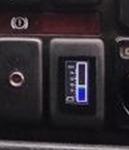
\includegraphics[width=.85\textwidth,height=.60\textheight,keepaspectratio]{figures/ivevo/image16.png}
\caption{Voltímetro}
\end{figure}

\begin{figure}[H]
\centering
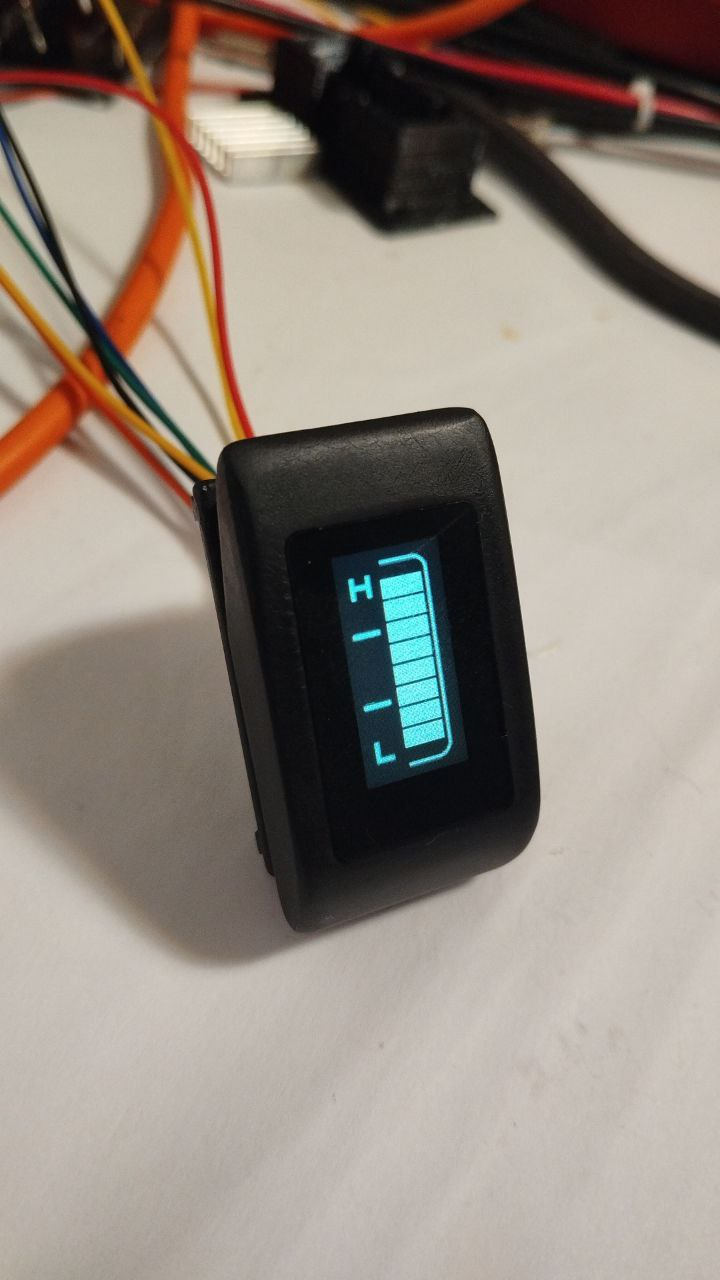
\includegraphics[width=.85\textwidth,height=.60\textheight,keepaspectratio]{figures/ivevo/image15.png}
\caption{Voltímetro}
\end{figure}

\begin{figure}[H]
\centering
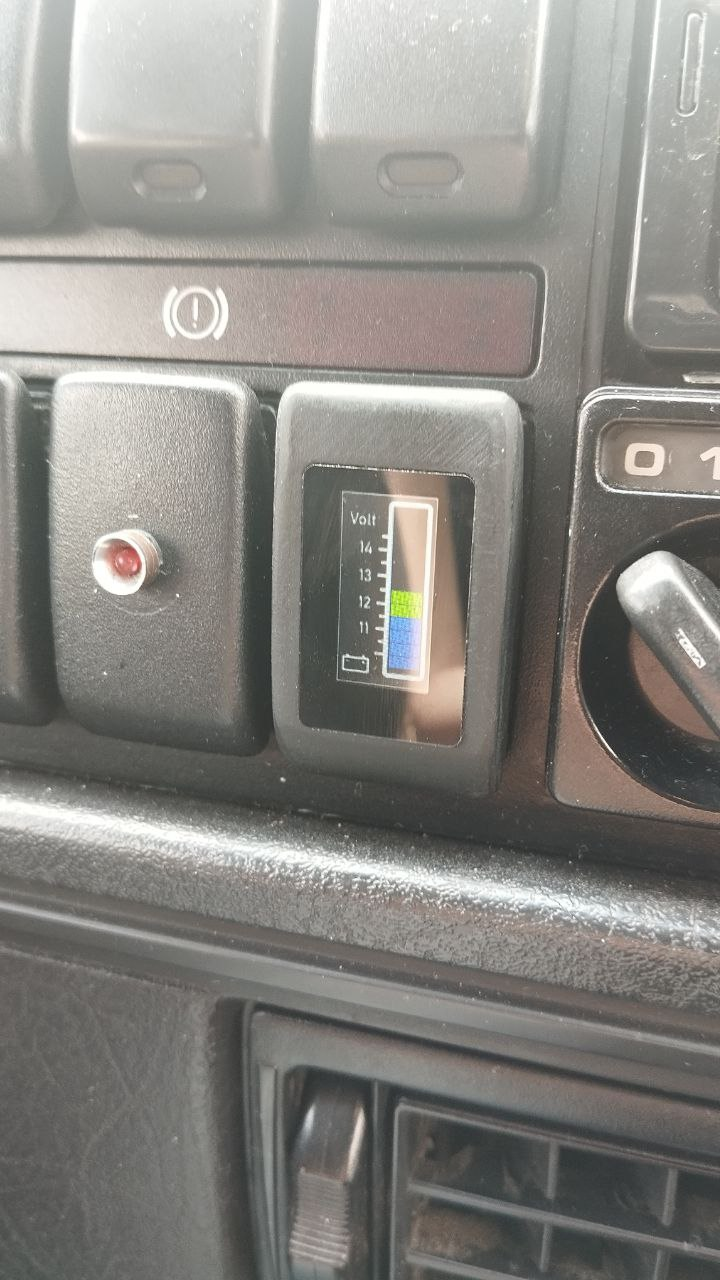
\includegraphics[width=.85\textwidth,height=.60\textheight,keepaspectratio]{figures/ivevo/image2.png}
\caption{Voltímetro}
\end{figure}
\section{Presión de aceite (Barometer)}
Requiere un sensor; el modelo previsto es VAG 03C906051A. Aunque IV-Evo dispone de +5 V, la fuente recomienda un convertidor DC/DC externo para alimentar el sensor. Siga el esquema de aceite y calibre según el sensor utilizado.

\begin{figure}[H]
\centering
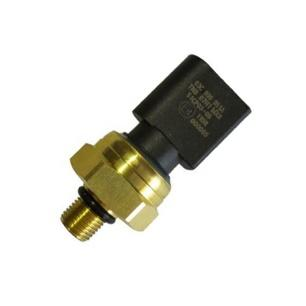
\includegraphics[width=.85\textwidth,height=.60\textheight,keepaspectratio]{figures/ivevo/image21.jpg}
\caption{Presión de aceite (Barometer)}
\end{figure}
\section{Temperatura (Thermo)}
Seleccione un NTC o un DS18B20 digital y el script correspondiente. Se admiten sondas DS18B20 con cable. Para NTC se recomienda Ossca 01176 o un sensor compatible de Golf 2. En el sensor Ossca, una los pines del sensor 1 y 2; la resistencia NTC se conecta al pin del sensor 3. Son números del sensor, no los pines de alimentación del indicador.

\begin{figure}[H]
\centering
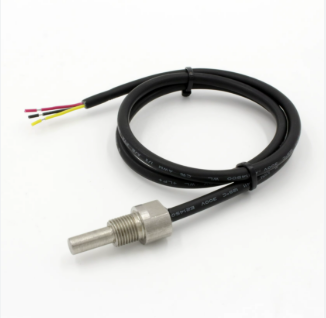
\includegraphics[width=.85\textwidth,height=.60\textheight,keepaspectratio]{figures/ivevo/image14.png}
\caption{Temperatura (Thermo)}
\end{figure}

\begin{figure}[H]
\centering
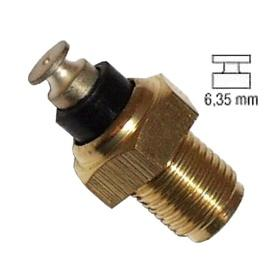
\includegraphics[width=.85\textwidth,height=.60\textheight,keepaspectratio]{figures/ivevo/image19.jpg}
\caption{Temperatura (Thermo)}
\end{figure}
\section{Indicador de marcha}
Admite R y marchas 1–5. Calcula la marcha a partir de velocidad y RPM recibidas de Digifiz Next por Bluetooth LE. La marcha atrás requiere una señal positiva en una entrada según el esquema. Se necesita firmware Digifiz Next 1.0.14 o posterior.

Para esta aplicación, conecte el pin 1 (K30/KL30) a +12 V KL15 bajo contacto y el pin 7 a masa. Al arrancar, un guion significa que no hay marcha seleccionada y el indicador busca Digifiz Next. Entre en el modo QR, seleccione iv\_gear y el sensor volts1, guarde y reinicie el contacto.

En el panel web de Digifiz Next ajuste la velocidad con GPS, las RPM y la tabla de marchas para el vehículo. La fuente propone 80–100 km/h como referencia; hágalo solo en condiciones legales y seguras, con un acompañante registrando los datos. Los valores de calibración de RPM 1500, 3000 y 400 no tienen unidades ni correspondencia inequívoca con motores. Consulte las instrucciones del cuadro para el motor concreto, sin adivinar valores.

\begin{figure}[H]
\centering
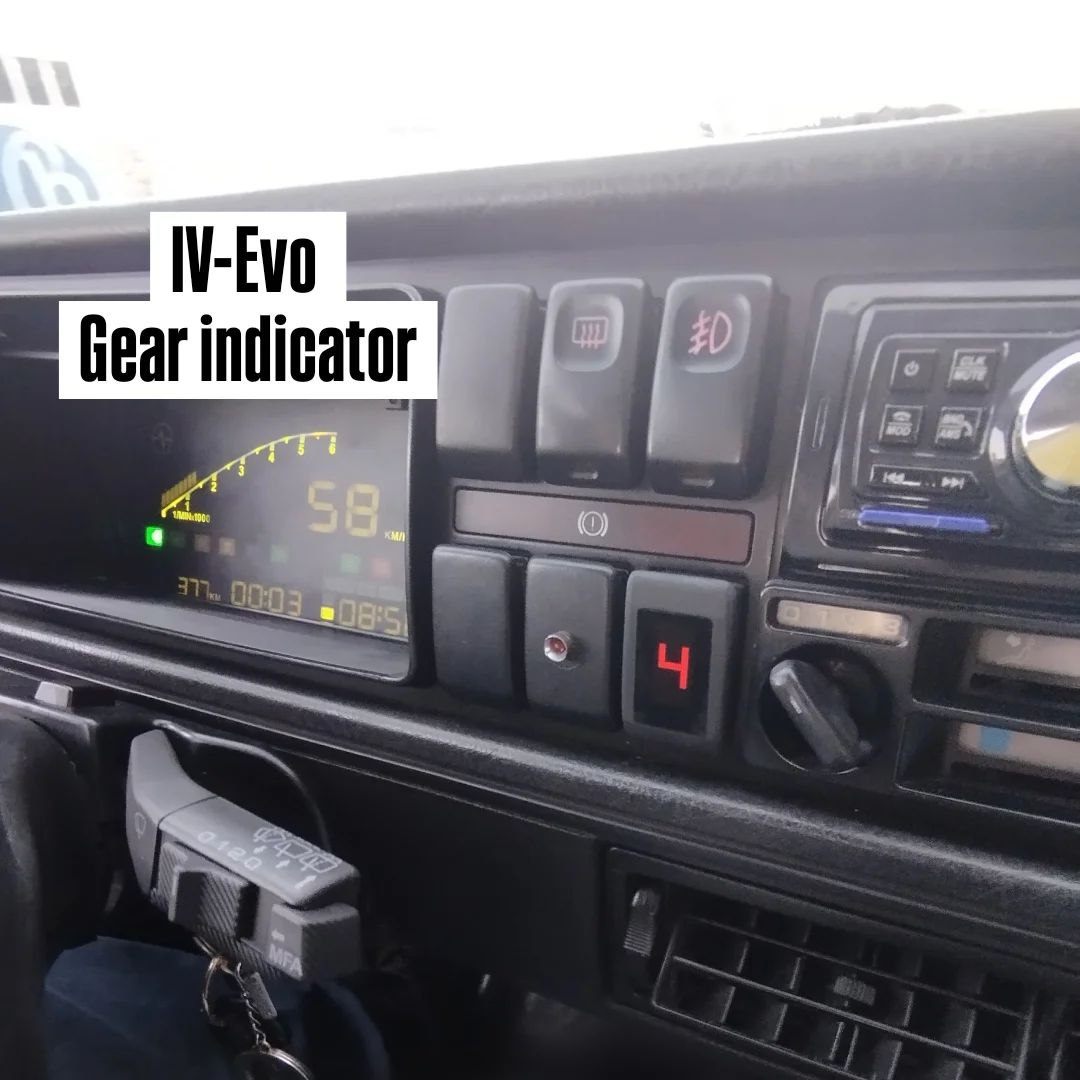
\includegraphics[width=.85\textwidth,height=.60\textheight,keepaspectratio]{figures/ivevo/image18.png}
\caption{Indicador de marcha}
\end{figure}

\begin{figure}[H]
\centering
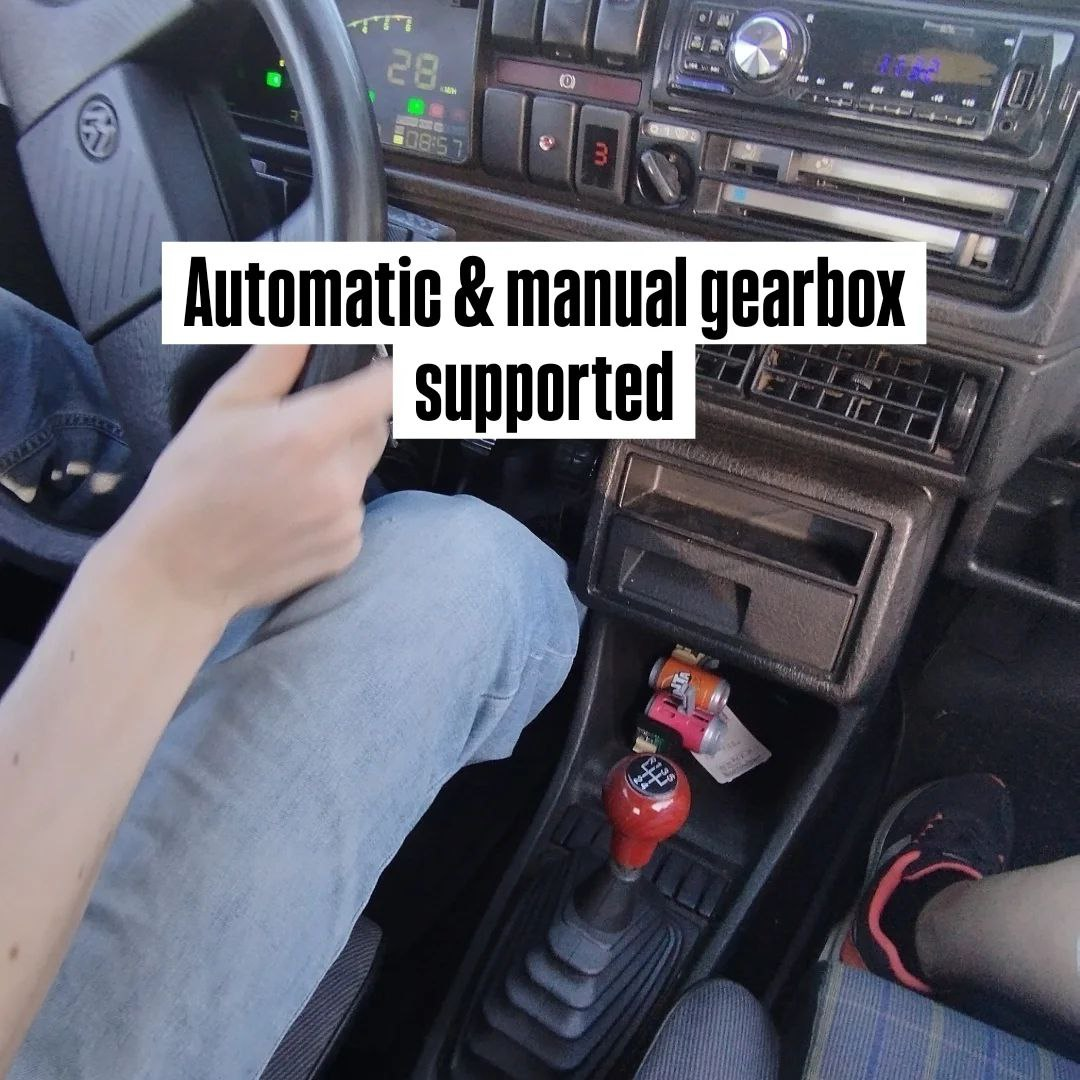
\includegraphics[width=.85\textwidth,height=.60\textheight,keepaspectratio]{figures/ivevo/image10.png}
\caption{Indicador de marcha}
\end{figure}
\section{Lambda}
No conecte el indicador a la sonda lambda original del Golf 2. La fuente exige una sonda de medición independiente; si conserva la original, habrá dos sondas. Una sonda de banda estrecha entrega aproximadamente 0,1 V (mezcla pobre) a 0,9 V (rica), sin medir con precisión la relación aire-combustible. Su conexión directa requiere calibración.

Una sonda de banda ancha necesita un controlador independiente; IV-Evo no puede controlarla directamente. Se recomienda Bosch LSU 4.9 con un controlador compatible, como SLC Free, DIY-EFI TinyWB, Sigma Lambda Controller Free 2 o rusEFI wideband. Conecte la sonda siguiendo las instrucciones del controlador y utilice su salida analógica. Puede ser 0–5 V, 0,5–4,5 V o 0–1 V; la conversión de entrada y la curva de calibración deben coincidir.

\begin{figure}[H]
\centering
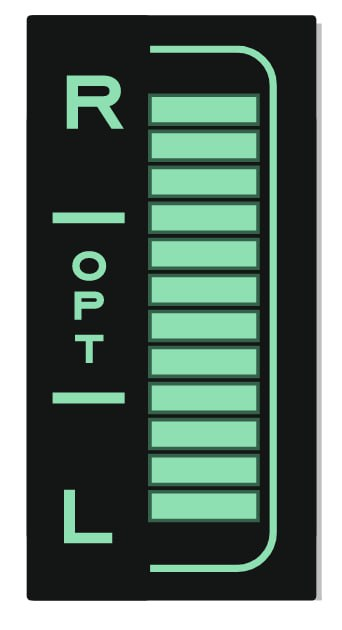
\includegraphics[width=.85\textwidth,height=.60\textheight,keepaspectratio]{figures/ivevo/image7.png}
\caption{Lambda}
\end{figure}
\section{Check Engine}
Muestra «Check Engine» con 12 V en el pin 2 (V2) y deja la pantalla vacía con 0 V. Es un indicador de señal; no se describe lectura de códigos ni interfaz OBD.

\begin{figure}[H]
\centering
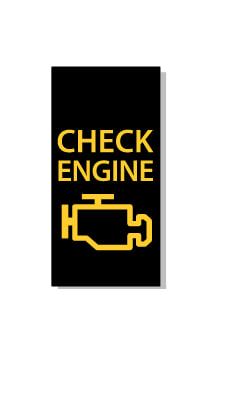
\includegraphics[width=.85\textwidth,height=.60\textheight,keepaspectratio]{figures/ivevo/image4.png}
\caption{Check Engine}
\end{figure}
\section{Presión de sobrealimentación (Boost)}
Se indica un sensor de tres pines, alimentación +5 V, un orificio de montaje y rango de 20–250 kPa. Su salida nominal es +1,8 V. No se proporciona la presión correspondiente ni la función de transferencia completa. Confirme el sensor y su curva antes de calibrar; no deduzca una pendiente a partir de un único valor.

\begin{figure}[H]
\centering
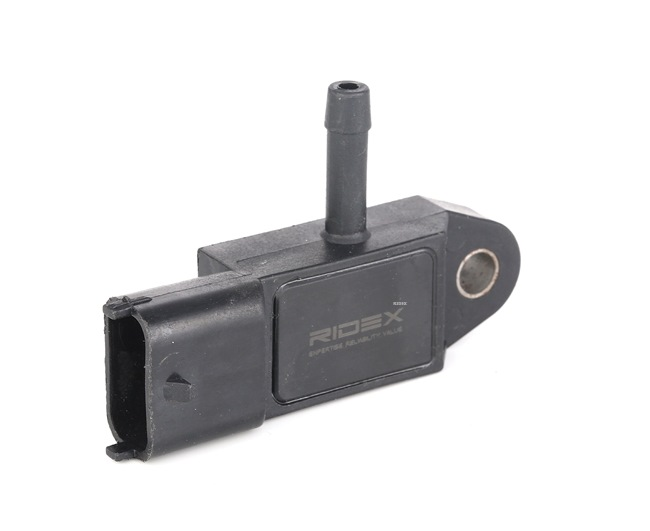
\includegraphics[width=.85\textwidth,height=.60\textheight,keepaspectratio]{figures/ivevo/image9.png}
\caption{Presión de sobrealimentación (Boost)}
\end{figure}
\section{Reloj}
La aplicación de ejemplo utiliza el reloj del sistema. La hora no se conserva al reiniciar; sin volver a ajustarla, funciona como contador del tiempo de viaje.

\begin{figure}[H]
\centering
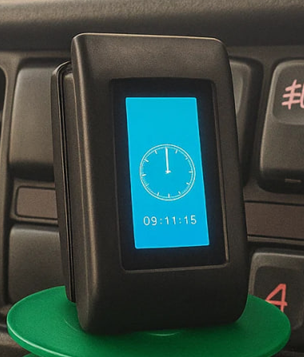
\includegraphics[width=.85\textwidth,height=.60\textheight,keepaspectratio]{figures/ivevo/image12.png}
\caption{Reloj}
\end{figure}
\section{Límites de la documentación}
No se especifican tolerancias generales de alimentación, temperaturas de trabajo ni grado de protección de la carcasa. No aplique a IV-Evo especificaciones de Nano.
